\documentclass[a4paper,12pt]{ctexart}

\usepackage{mathtools}
\usepackage{amsmath}
\usepackage{cleveref}
\usepackage{amssymb}
\usepackage{geometry}
\usepackage{enumitem}
\usepackage{tabularx}
\usepackage{color}
\usepackage{float}
\usepackage{geometry}
\geometry{top=3cm,bottom=3cm}
\usepackage{ulem}
\usepackage{fancyhdr}
\pagestyle{fancy}
\renewcommand{\headrulewidth}{0pt}
\fancyhead{}
\fancyfoot[C]{\thepage}

\usepackage{titlesec}
\titleformat*{\section}{\centering\heiti\zihao{4}}
\usepackage{zhnumber}
\renewcommand\thesection{\zhnum{section}、\hspace{-1em}}
\renewcommand\thesubsection{\arabic{section}.\arabic{subsection}}

\usepackage{amsmath}
\usepackage{graphicx}

\begin{document}
    \begin{figure}[h]
        \centering
        
\includegraphics[scale=0.6]{figures/封面.png}
    \end{figure}
    \begin{center}
        题目:\uline{A题:路口信号灯实时智能控制方案研究}
    \end{center}
    \begin{center}
    摘\qquad 要
\end{center}
\qquad 对路口信号灯实时智能控制方案研究分为了三部分,首先需要根据视频文件,进行图像识别,导出11:00至11:30的路口车辆的时间、大小,位置等信息。问题一需要统计视频中所有出现车辆的16项数据,需要运用计算机视觉领域的算法,属于图像识别和目标检测任务。我们先将视频转换为逐帧的图片序列。首先我们需要识别图像中的监控时间和红绿灯秒数,由于每个路口的监控时刻和红绿灯秒数在图像中的位置固定,因此我们人为地框定需要识别数字的区域。我们使用基于opencv实现的传统数字图像处理算法,结合基于 MNIST 预训练的 Resnet18 神经网络共同完成数字识别任务,当两种算法结果不一致时再人工纠正。其次我们检测图像中出现的车辆,我们使用在 coco 数据集上预训练的 tiny-YOLOv3 神经网络逐帧检测每张图像中的车辆,输出每辆车的 Bounding Box,并使用链接算法将帧与帧之间车辆的 Bounding Box 链接形成车辆轨迹。最后,我们使用投影算法测算图像中对应点位的实际距离。我们建立了若干蒙版(车道蒙版、路口蒙版、距离蒙版)用于识别 Bounding Box 所处的位置和离停车线的距离。
在求得第一问数据的基础上,我们得出了路口半小时内总流量为732辆,东西南北口分别为:217、202、120、193.平均速度为0.8290m/s.

交通信号灯先进行周期和相位划分,南北方向直行、南北方向左转、东西方向直行、东西方向左转分别为一二三四相位,总周期长为113秒。我们认为每个周期相互独立,分别求取周期内的阻碍时间。对于阻碍行为的定义中,我们只考虑相邻时间区间的阻碍行为。只存在直行阻碍同向的左转,以及左转阻碍异向的直行,两种情况,在实际考虑相位时,有四种含方向的阻碍类型。
阻碍时间的具体计算思想为:以双向车道中最后一辆车驶离停车线的绿灯显示时间为该相位车道阻碍另一相位的阻碍时间,与另一相位在最后一辆车辆驶离时刻之前已在停车等待的停车数量乘积结果为该相位的阻碍时长,再将四个相位结果相加,最终的阻碍时间为:
第三部分是信号灯配时优化问题。

第三问主要是信号灯时配的优化问题。首先对现有数据进行预处理,计算出各周期不同相位实际流通量,并依据该信息将总时间段按照不同相位特征分为三个子时间段。以减少平均延误、进入速度损失、增大通行能力为目的,构建目标函数。优化方法采用传统的Webster算法和遗传算法,求得最优周期和各相位有效绿灯时长。在此基础上再次输出进入车辆信息进行流通模拟,得到更新后的表格,并和原有信息进行对比分析。结果发现优化方案均能提高通过路口的平均速度,遗传算法所得结果效果更好。

关键字:图像识别;目标检测;Webster算法;遗传算法;交比
    \newpage
    \section{问题重述}\label{sec:peoblem_restatement}

本文研究的是路口信号灯实时智能控制方案研究,需要针对目前的红绿灯时长固定的机械转换方案进行改进。在车流量很大的路口,车辆排队进行等待的情况下,交通信号灯发挥着维持交通秩序的功能;但在车流稀少的情况,如果驾驶员沿东西方向行驶,此时南北方向无车驶过,如果没有交通信号灯,那么不需要减速即可通过路口,但在机械方案下,驾驶员需要减速停车等待半分钟以上的红灯,此时的交通信号灯显然阻碍了交通情况。此种阻碍,一方面增加了燃油量和碳排放,一方面影响了司机的心情和时间。

本文旨在,针对车流稀少的情况下,通过图像识别的方法,获取时间、车辆位置等信息,通过数据得到该路口诸如车流量、平均速度等基本信息,通过对交通灯阻碍交通的情况进行调查和分析,基于现状给出实时控制信号灯的智能方案,最大程度提高路口的车辆的通行速度。

我们需要依次解决如下问题:(1)通过图像识别,对于提供的视频素材,通过观察信号灯的显示时间,视频记录的时间,汽车在图片中位置信息及其动态变化等等,提取出车辆进入、停车、驶离的种种信息。(2)通过数据处理,根据识别得出的信息,计算一下该路口的总体指标,例如车辆通过该路段的总流量以及平均速度。给出阻碍行为的具体定义和算法,并且计算阻碍交通情况的总时间。(3)通过对路口优化方案的思考,以最大程度提高车辆通过路段的平均速度为目标,给出优化后的信号灯智能方案,并且根据新的方案,根据识别出的车辆进入信息,重新计算车辆的进出时间、进出距离等指标,计算出优化后的车辆的平均速度。

本题目的重心首先在于图像识别,图像可以识别出时间以及地理位置类信息,同时还要对图像识别的准确性进行优化,再进行图像坐标与世界坐标的变换求出图像中的距离信息。其次在于阻碍行为将一个相位的车辆数据与其他相位的数据联系在一起,在不同的相位考虑相互的阻碍,定义和算法都略难梳理。最后信号灯配时问题,适配车辆稀少情况下的配时算法研究的较少,故对算法的修正也是重点。

    \section{变量解释、前提和假设}\label{sec:hypothesis}

\subsection{辅助说明}\label{subsec:hypothesis-description}

题干中给出了许多关于路面状况的信息作为辅助说明,我们首先需要对其进行理解。因为世界是三维的,而图片是二维的,故首先需要将给出的三维中的数据信息在二维图像中直观表示,这样便于我们理解。首先我们对路口的平面图进行数据的简单标注,如图\ref{fig:p1}所示。

\begin{figure}[h]
    \centering
    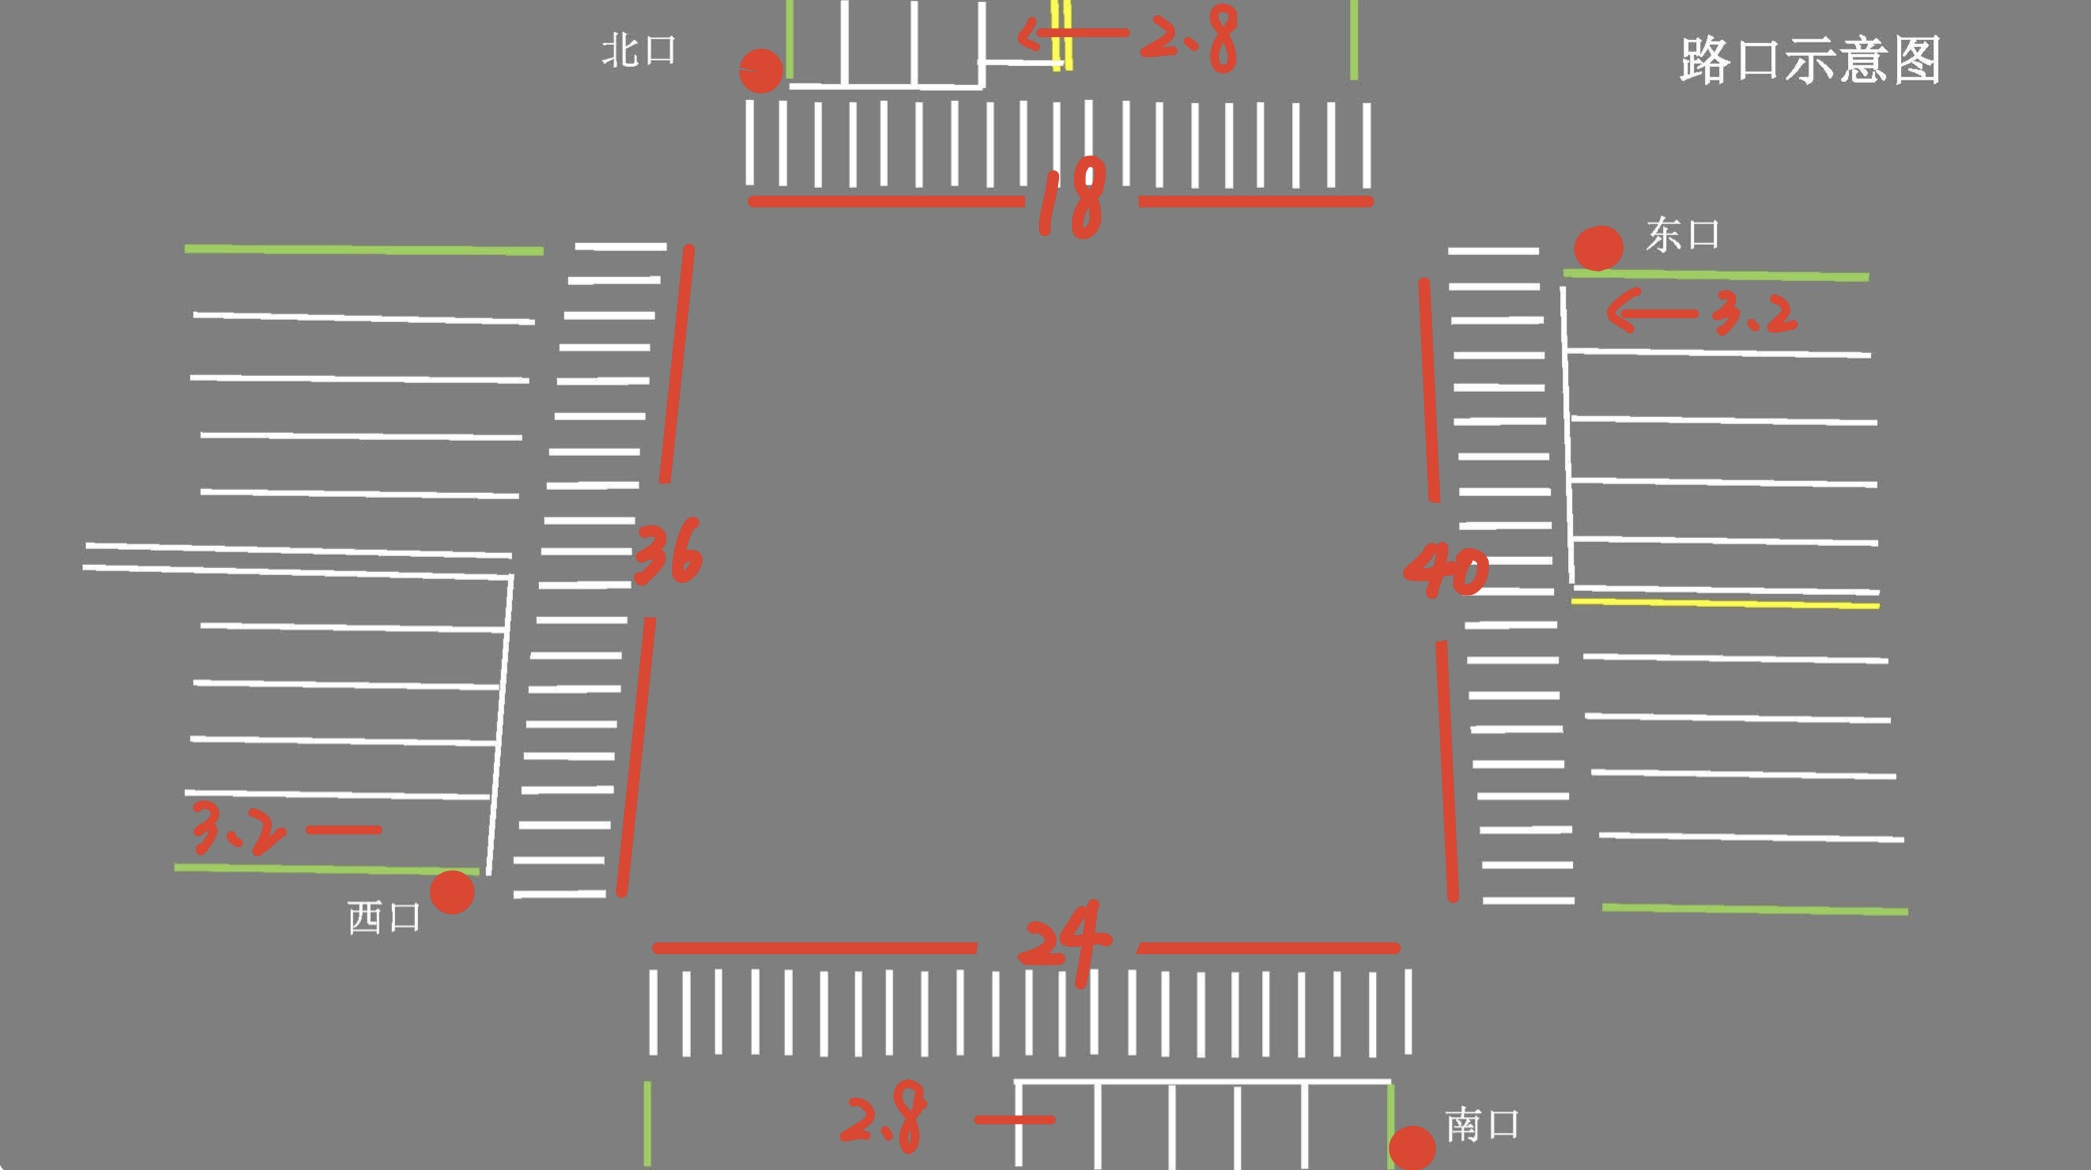
\includegraphics[scale=0.1]{figures/路口阴影图.jpg}
    \caption{路口平面图}
    \label{fig:p1}
\end{figure}

以南口为例,绿线之内为除人行道以外的车道,南口的绿线内总长度为24米,每一个机动车道宽为2.8米。摄像机的位置为图中红点的位置,大致位于路面右侧,交通灯位于对面路的左侧。可以发现,该路口并非一个规则的四边形结构,不仅各边长度不同,各边之间还呈现不同的角度。

考虑到实际生活中的路口形状,不仅有图\ref{fig:p1}所观察出的不规则四边形的特征,还有可能存在诸如在路的拐角出会存在比较大的空白区域这样的问题。考虑了这些因素,我们对图一进行了优化,通过对视频中的路的名称的提取,我们在地图中寻找友谊河路与石杨路交叉路口,通过地图的测距功能得到有关该路口更精确的数据。如下图所示:

\begin{figure}[h]
    \centering
    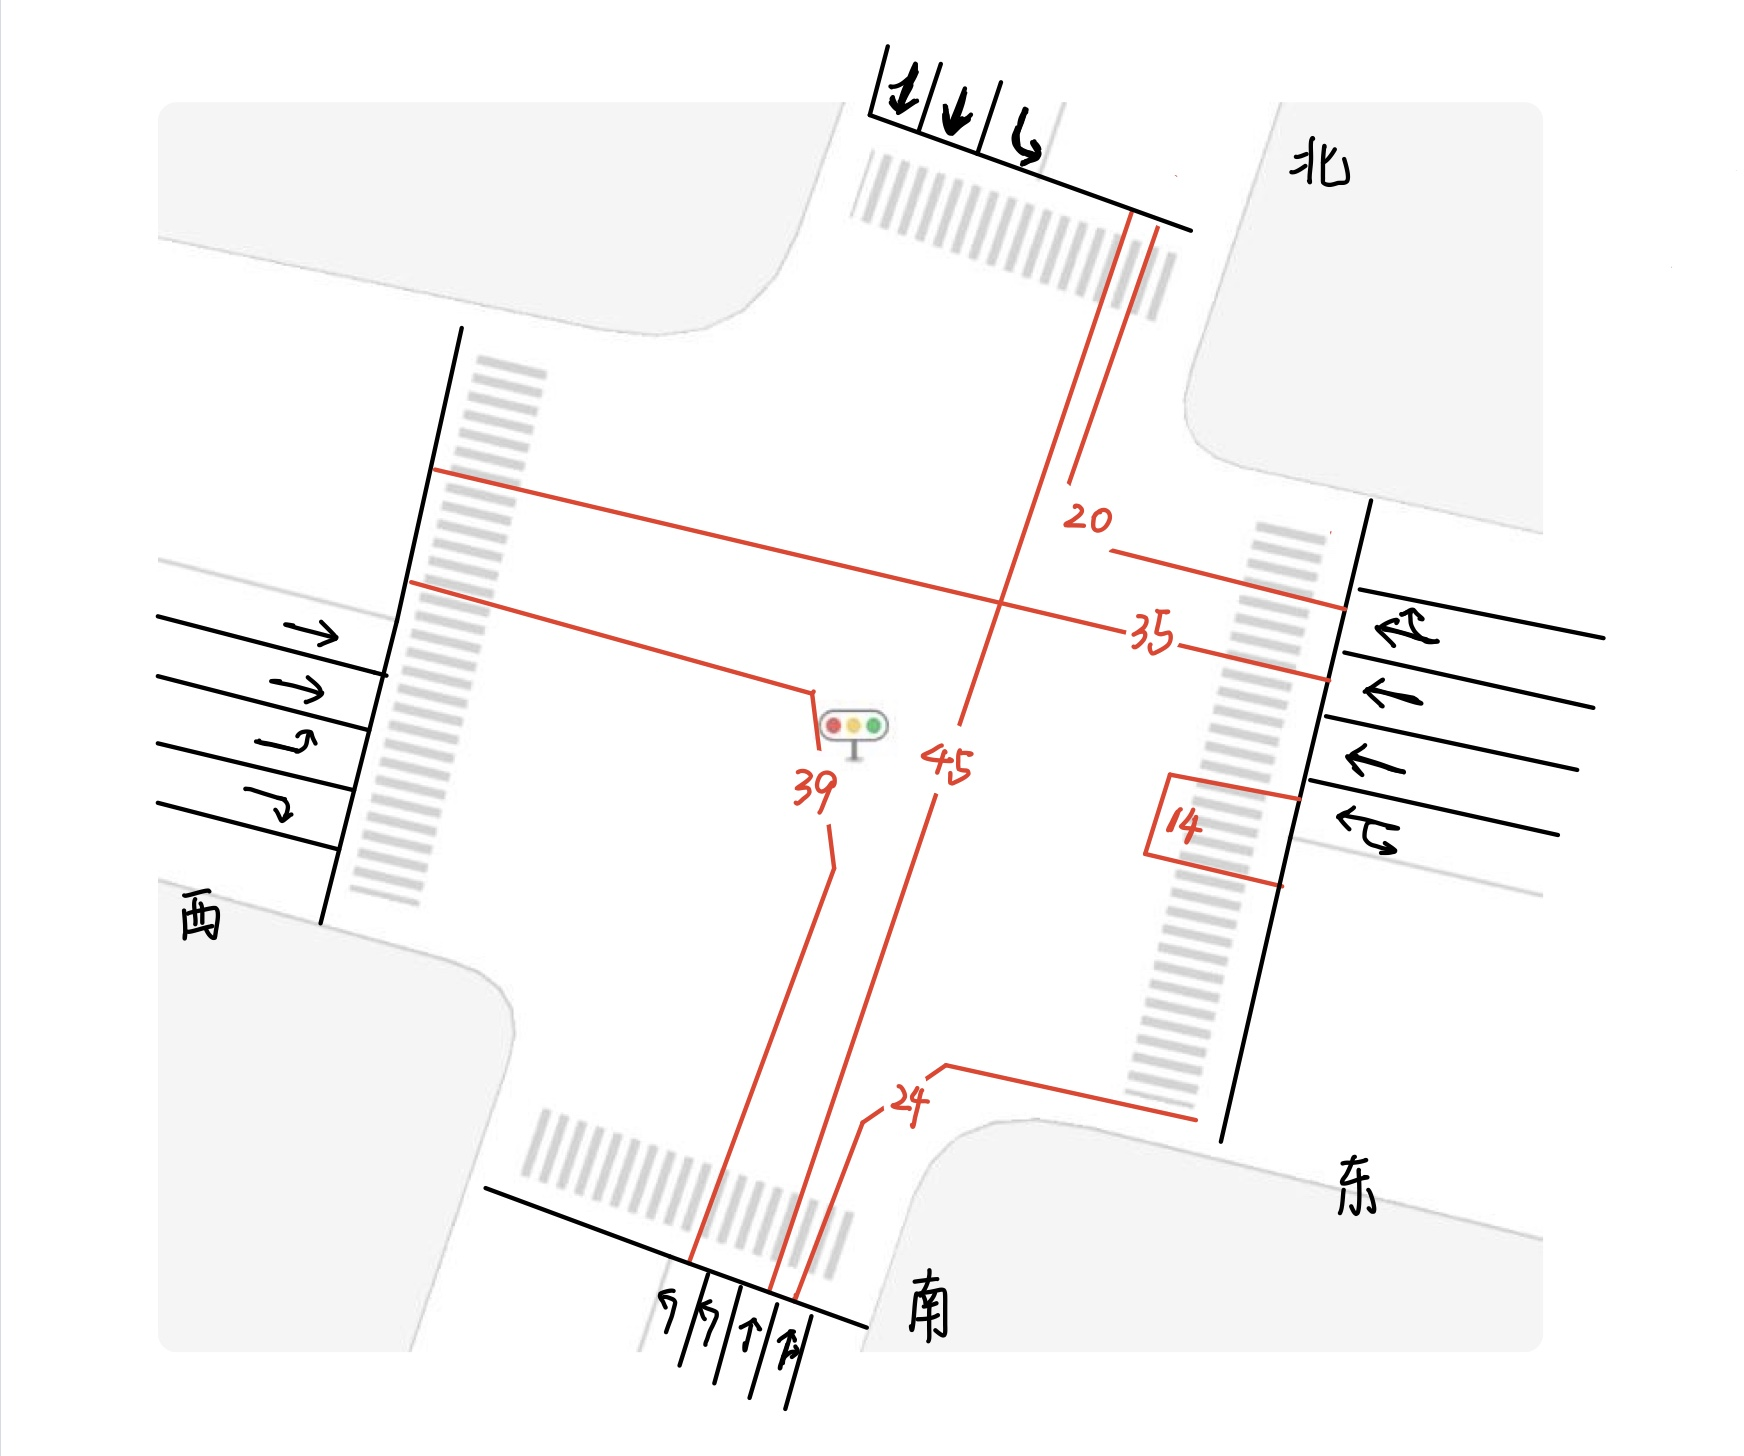
\includegraphics[scale=0.15]{figures/路口平面图.jpg}
    \caption{轨迹距离图}
    \label{fig:p2}
\end{figure}

如\ref{fig:p2}所示,相比上图,显而易见,出现了四个较大面积的拐角,我们将每个路口的行车指示标注其中,粗略测量出了南北方向的停车线之间的长度约为45米,由南口左转至西口停车线的距离约为39米,右转至东口停车线的位置约24米。自东口掉头穿过斑马线的距离约为14米,自东口驶向西口的直线距离约为35米,自东口右转至北口的距离约为20米。收集这部分数据是因为,在车辆位置的判定中,车辆远离停车线30米以上,就视为车辆离开了路口。有了关于路口更精确的数据,可以找到具体处于哪一位置时,视作车辆离开路口。

通过该图,可以简要说明为车道编号的过程中。编号均以最靠中间隔离物的车道为第一车道,以图\ref{fig:p2}的南口为例,最左侧左转车道为南1,第二个左转车道为南2,直行车道为南3,直行加右转车道为南4。

有一些关于摄像机以及路灯高度的数据,我们截取了南口含摄像机的图片,如下所示:

\begin{figure}[h]
    \centering
    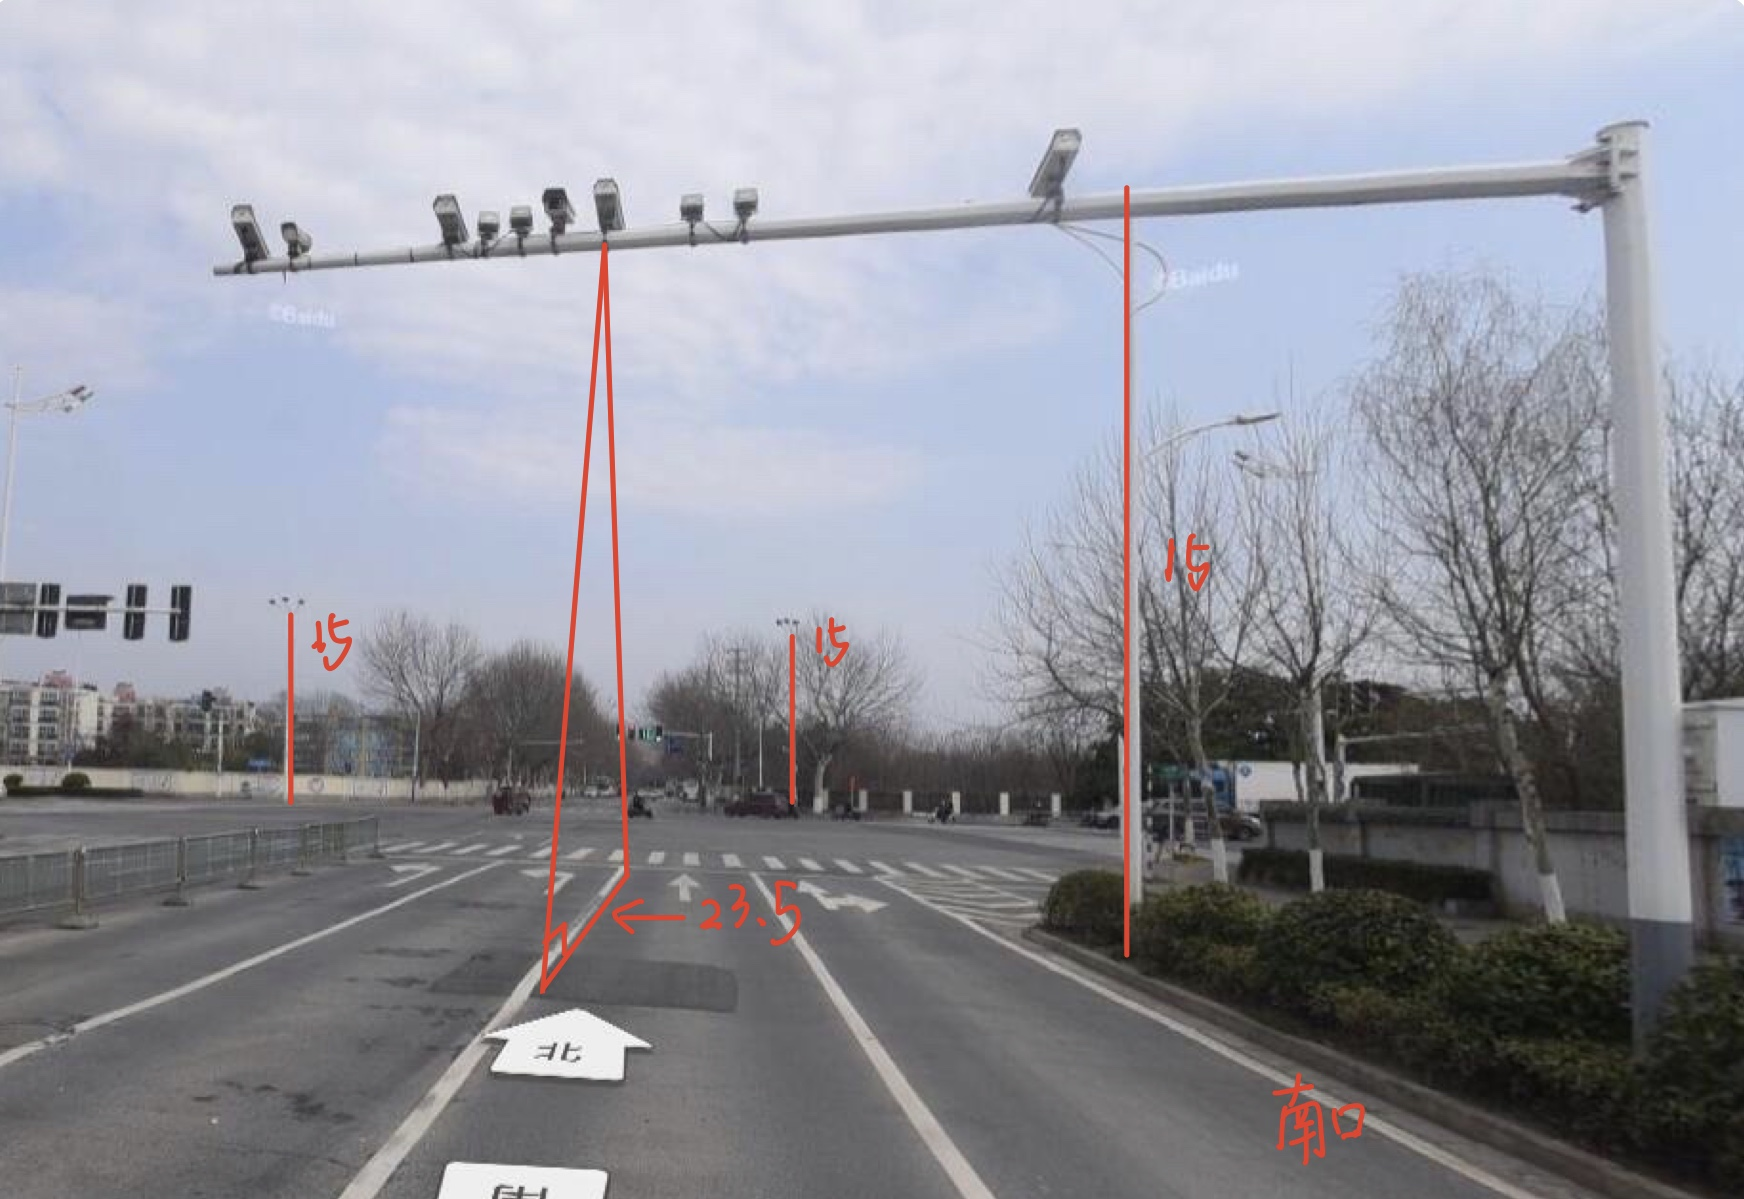
\includegraphics[scale=0.15]{figures/摄像机位置图.jpg}
    \caption{摄像机位置图}
    \label{fig:p3}
\end{figure}

如\ref{fig:p3}所示,这是一张摄于南口的图片,摄像头离地面的高度为6米,自摄像机位置向地面做铅垂线,与地面的交点向停车线作垂线,该垂线即为摄像头的铅直投影点到停车横线的距离,在图中,南口该位置处的距离为23.5米,路口四角处的路灯均为15米高。这些数据,均可用于图片距离向实际距离转化时的参照物。

剩余的辅助说明较好理解,这里作简要介绍。

1.除四角大路灯外,道路上的路灯间距为40米,北口和南口的路灯高10米,东口西口高12米。

2.车辆编号依时间顺序进行,若同时出现,则自画面左侧向右编号,即靠近道路中轴线先编号。

3.车辆位置是指车头距离停车横线的距离,到达停车横线之前为正距离,驶离时为负距离。若车辆驶离停车线30米以上将不再记录距离。

4.车辆的大中小行分类是依据“car”“truck”“bus”标签进行分类的。

\subsection{变量解释}\label{subsec:hypothesis-variables}

通过在视频中的一帧截屏展示的数据,我们对所需要收集的15个变量进行讨论。还有一点要注释的,在附件提供的视频中,视频已经在原基础上5倍速播放。

\begin{figure}[h]
    \centering
    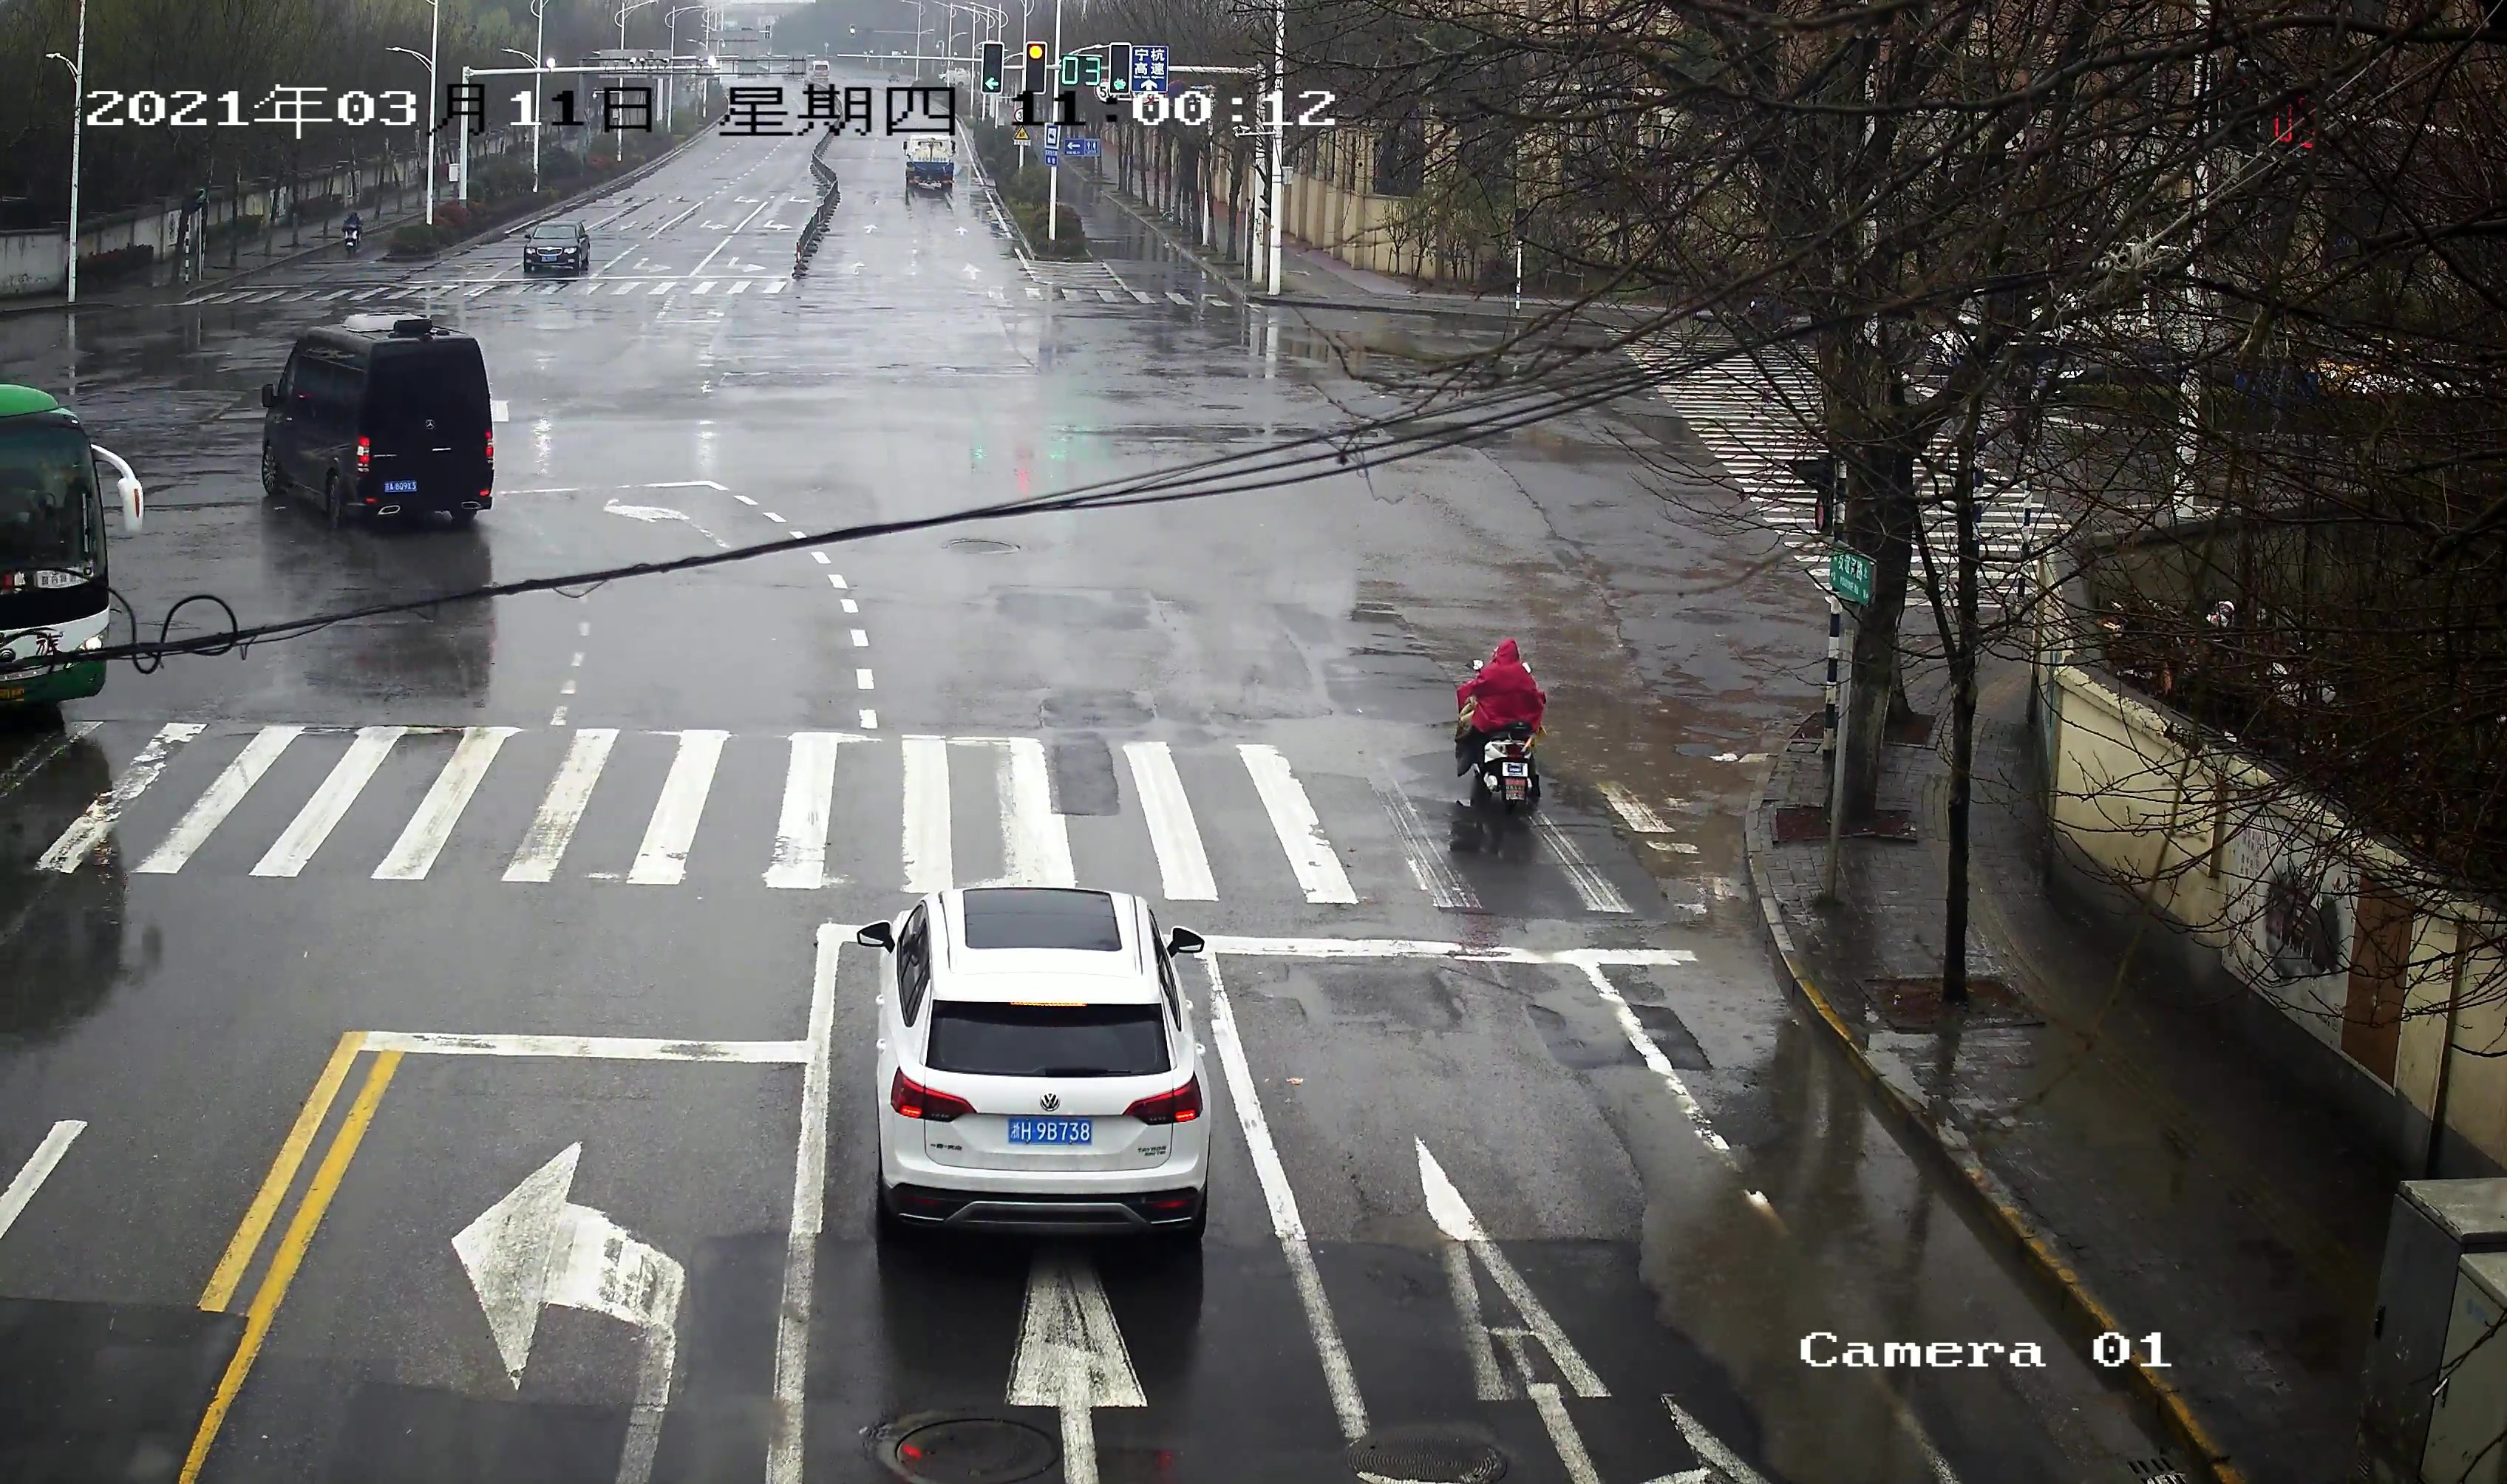
\includegraphics[scale=0.1]{figures/视频截图.jpg}
    \caption{北口视频截图}
    \label{fig:p4}
\end{figure}

如图\ref{fig:p4}所示,左上角有精确的日期和时间的数据,若有车辆从下框进入,即可确定进"进入时刻","进入车道","进入位置",若此时正值红灯,那么车辆在停车线出静止时即可获得"停车时时刻","停车车道","停车时位置","停车时红灯显示时间"等变量,若此时正值绿灯,则这些变量数据为空。

车辆驶离的判定标准为驶离路口30米以上。可以依据前面的手工测量数据,确定驶离位置。以由南向北直行的车辆考虑,行驶至两个停车线距离的$30/45=2/3$时,即可认为是驶离路口。由位置可以确定"驶离路口横线时刻","驶离横线时车道"即为车辆的驶入车道,"驶离横线时绿灯显示时间"和"驶离路口时刻"可由视频时间得出。

进出时间长度由"进入时刻"与“驶离路口横线时刻”作差得出。“进出距离长度”,可由进入位置与驶出位置的轨迹长度确定。

\subsection{前提和假设}\label{subsec:hypothesis-premise}

\begin{figure}[h]
    \centering
    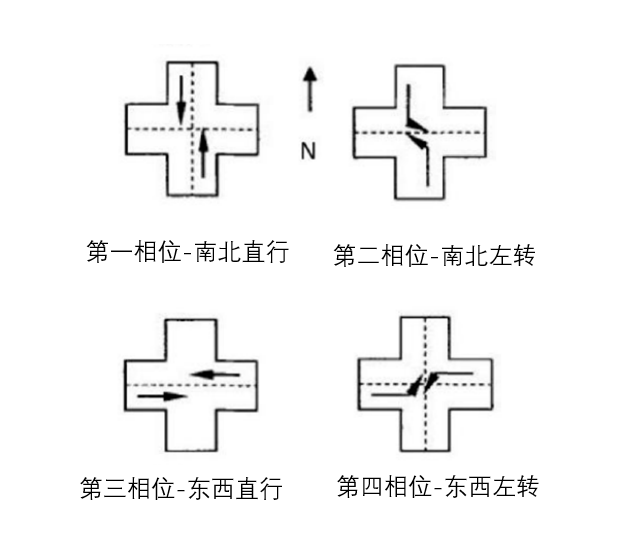
\includegraphics[scale=0.5]{figures/四相相位图.png}
    \caption{相位示意图}
    \label{fig:相位}
\end{figure}

在对于交叉路口的研究中,通常采用四相位控制,本文依照惯例采用如\ref{fig:相位}所示的四相位:东西直行、东西左转、南北直行、南北左转。

在此部分,我们对全文的通用假设进行说明:

(1)任何时候右转的车辆都是可以右转的,对于右转方向的车流,认为其对其他方向的交通流没有影响,在四相位的交通流中,左转方向的交通流,其对整个交通流的影响较大。

(2)在视频中,存在车辆掉头的行为,在本文对于阻碍交通问题的研究中,我们将掉头行为认同为左转,因为和左转需要等待的时间相同,并且驶离路口所用时间和距离接近。

(3)在对路口状况进行抽象建模的过程中,我们可能认为每个周期车辆的到达服从泊松分布。

(4)在本文中识别的路口,由于车辆驶入不含摄像头的一侧,故认为所有识别的车辆不存在数据重合的可能。

(5)本文不考虑行人以及非机动车的影响。

    \section{问题一建模}
在问题一中,我们需要对视频中的车辆的15个指标进行识别和记录,此处需要用到图像识别的方法,对于时间类变量,对视频左上角的时间,信号灯的秒数,车辆的位置等等进行识别即可获得;但对于距离类或者速度类变量,还需要涉及将图片中的距离转化为实际距离这一步骤。问题一模型的核心由这两部分构成。

\subsection{图像识别}

\subsubsection{时间识别}
在本题中,时间的识别包含两个部分,一个是视频左上角的时刻,一个是信号灯倒计时的秒数。想要识别图像字符,需要模板库,在此处我们应用自己训练的数据集。

首先将图片进行灰度处理,

低于某一数值变成白色,高于某一数值变成黑色,最终得到第三行数据,然后根据该行信息,与前一张图片的信息作差,得到第四行数据,没有信息差的图片呈现为黑色,有信息差的会有不规则图像的出现。通过该信息我们可以得知,在何时秒数跳动。(传统的方法)
对于视频中存在的视频不连贯的问题(比如跳帧从6秒到8秒)那么传统方法不灵验,故采用神经网络的方法进行识别。

\subsubsection{车辆识别-YOLO算法}

YOLO将单个神经网络应用于完整图像,将图像划分为多个区域并预测每个区域的边界框和概率。YOLO检测网络包括24个卷积层和2个全连接层,卷积层用来提取图像特征,全连接层用来预测图像位置和类别概率值。
\begin{figure}[h]
    \centering
    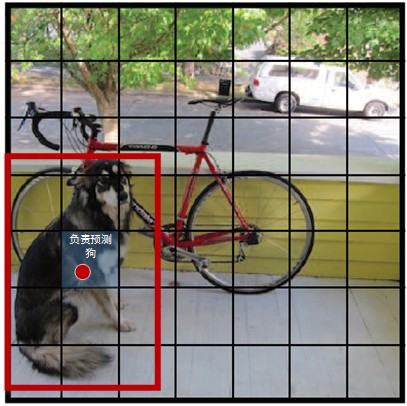
\includegraphics[scale=0.5]{figures/YOLO网格.png}
    \caption{YOLO网格示意图}
    \label{fig:YOLO}
\end{figure}

如\ref{fig:YOLO}所示,YOLO的CNN网络将输入图像分为$S\times S$个网格,每个格子负责检测中心点落在该格子内的目标。若某个物体的中心位置的坐标落到了某个格子,如格点图所示,狗的中心位置位于左下方格点处,那么这个格子就负责检测出这个物体。每个单元格会预测B个边界框以及边界框的置信度。置信度包含两个方面的信息,即边界框含有目标的可能性的大小和边界框的准确度。前者记为$Pr(object)$,若边界框不含物体取值为0,完整包含物体取值为1.准确度信息是用边界框与物体真实区域的交集面积(该面积以像素为单位),记为$IUO^{truth}_{pred}$。置信度的最终定义为$Pr(object)*IUO^{truth}_{pred}$。


边界框的大小和位置可以用4个值来表示(x,y,w,h)。其中(x,y)是边界框的中心坐标,(w,h)是边界框的宽与高。
其中(x,y)是相对于每个单元格左上角坐标点的偏移值,并且单位是相对于单元格大小的,边界框的宽和高是相对于整个图片的宽和高的比例,故四个元素的大小应该 均在[0,1]范围内。
同时每一个单元格需要预测出C个类别概率值,由该单元格负责的边界框其目标属于各个类别的概率。


每个单元格的预测需要$(B*5+C)$个值,如果将输入图片划分成$S*S$网格,那么最终的预测值为$S*S*(B*5+C)$大小的张量。
\begin{figure}[H]
    \centering
    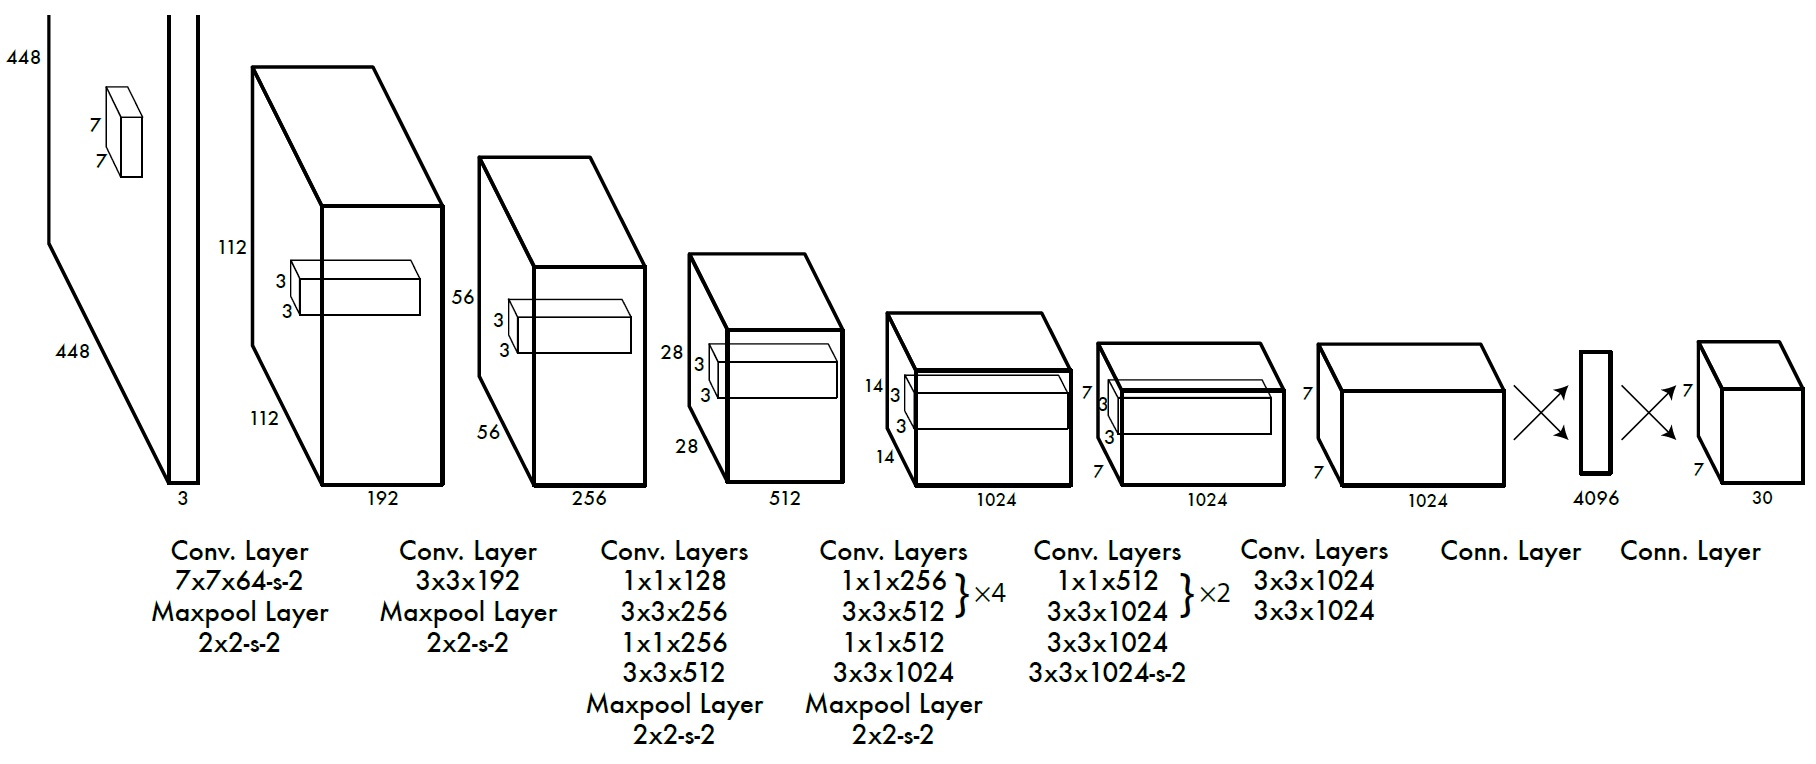
\includegraphics[scale=0.1]{figures/网络结构.jpg}
    \caption{网络结构示意}
    \label{fig:网络}
\end{figure}
Yolo采用卷积提取特征,使用全连接层得到预测值。具体形式可参考下图\ref{fig:网络},如图所示,对于卷积层,主要使用$1 \times 1$卷积来做channle reduction,然后紧跟$3 \times 3$卷积。对于卷积层和全连接层,采用Leaky ReLU激活函数:$max(x,0.1x)$,最后一层采用线性激活函数。

YOLO将目标检测看成回归问题,采用的是均方差损失函数。但对不同的部位采用了不同的权重值。定位误差即边界框坐标预测误差的权重值为5;不包含目标的边界框的置信度权重值为0.5;含有目标的边界框的置信权重为1。实际上较小的边界框坐标误差应该比大的边界框更敏感。为了保证这一点,将网络的边界框的宽与高预测改为对其平方根的预测,即预测值变为$(x,y,{\sqrt{w}},\sqrt{h})$
损失函数为:
\begin{equation}
    \begin{aligned}
        &\lambda_{\text {coord }} \sum_{i=0}^{S^{2}} \sum_{j=0}^{B} \mathbb{1}_{i j}^{\text {obj }}\left[\left(x_{i}-\hat{x}_{i}\right)^{2}+\left(y_{i}-\hat{y}_{i}\right)^{2}\right] \\
        &\qquad \begin{aligned}
                    +\lambda_{\text {coord }} \sum_{i=0}^{S^{2}} \sum_{j=0}^{B} \mathbb{1}_{i j}^{\text {obj }}\left[\left(\sqrt{w_{i}}-\sqrt{\hat{w}_{i}}\right)^{2}+\left(\sqrt{h_{i}}-\sqrt{\hat{h}_{i}}\right)^{2}\right] \\
                    +\sum_{i=0}^{S^{2}} \sum_{j=0}^{B} \mathbb{1}_{i j}^{\text {obj }}\left(C_{i}-\hat{C}_{i}\right)^{2} \\
                    +\lambda_{\text {noobj }} \sum_{i=0}^{S^{2}} \sum_{j=0}^{B} \mathbb{1}_{i j}^{\text {noobj }}\left(C_{i}-\hat{C}_{i}\right)^{2} \\
                    +\sum_{i=0}^{S^{2}} \mathbb{1}_{i}^{\text {obj }} \sum_{c \in \text { classes }}\left(p_{i}(c)-\hat{p}_{i}(c)\right)^{2}
        \end{aligned}
    \end{aligned}
\end{equation}
其中第一项是边界框中心坐标的误差,第二项是边界框的高与宽的误差项,第三项是包含目标的边界框的置信度的误差项。
我们插入一张YOLO算法得到的结果图\textcolor{red}{插入结果图},如下:
(通过该算法,我们可以得到包含目标物体的框,并且有标注-car truck-person等信息。)

\subsection{距离转换}

\subsubsection{基于相机模型的坐标简介}
相机的拍摄实际上是一个透视过程,在本文的研究中我们用小孔成像模型来研究相机成像。

从计算机视觉的视角,一张图片我们需要考虑多个坐标系:

(1)以相机光心O组成的坐标系称为相机坐标系$O_c-X_c-Y_c-Z_c$;X轴与Y轴分别平行于图像坐标系的X轴和Y轴,Z轴为相机的光轴方向。

(2)以光心在相平面投影$O'$(图像平面中心)为原点的坐标系称为图像坐标系$O-X-Y$;

(3)以图像左上角为原点的坐标系称为像素坐标系$O-u-v$;像素坐标系的两轴分别平行于图像平面的两条垂直边。

(4)物体在真实世界的坐标用世界坐标系来描述$O_w-X_w-Y_w-Z_w$.
我们在博客中找到了下图,可以清晰的表示坐标系间的关系:
\begin{figure}[H]
    \centering
    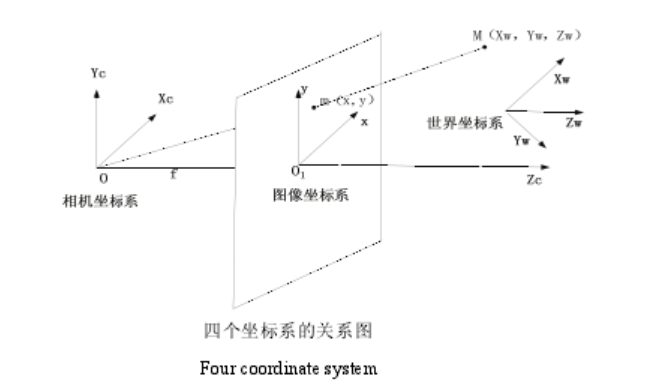
\includegraphics[scale=1]{figures/坐标系相互关系.png}
    \caption{坐标系相互关系}
    \label{fig:p5}
\end{figure}

\subsection{相机成像的性质}
在现实生活中,平行的线永不相交,但在照片中,平行的马路不再平行,看似会在远处交于一点,所以照片中的数据性质需要重新进行研究,图像坐标系下的部分距离信息与世界坐标系下并不相一致。

性质1:摄像头把平行的直线映射为图像上的相交直线,这个交点被称为消隐点(vanish point)。所有的平行的直线都各自交于无穷远处的一点,这些点会构成无穷远直线,这条线被称为plane vanishing line-消失的地平线.
\begin{figure}[H]
    \centering
    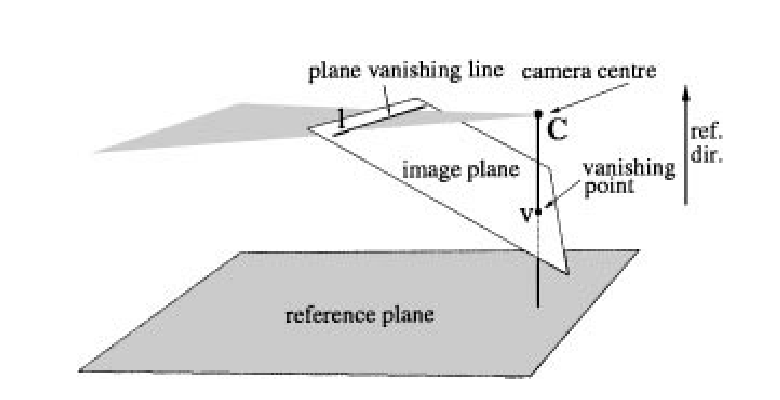
\includegraphics[scale=1]{figures/相机成像.png}
    \caption{相机成像}
    \label{fig:p6}
\end{figure}
这一图片来自论文\textcolor{red}{某篇论文},其中reference plane代表地面,image plane则是相机所拍出的照片,C点为相机的中心点。消失的地平线是由过C点且与地面平行的平面与照片的交线。

性质2:摄像头把三维空间投影到二维图像上,保持直线交比不变。交比是四个点两两“比例的比例”。如果在三维空间中有一条直线上有4个点,那么它们映射到图片上的四个点后,四个点的交比不变。


\begin{figure}[H]
    \centering
    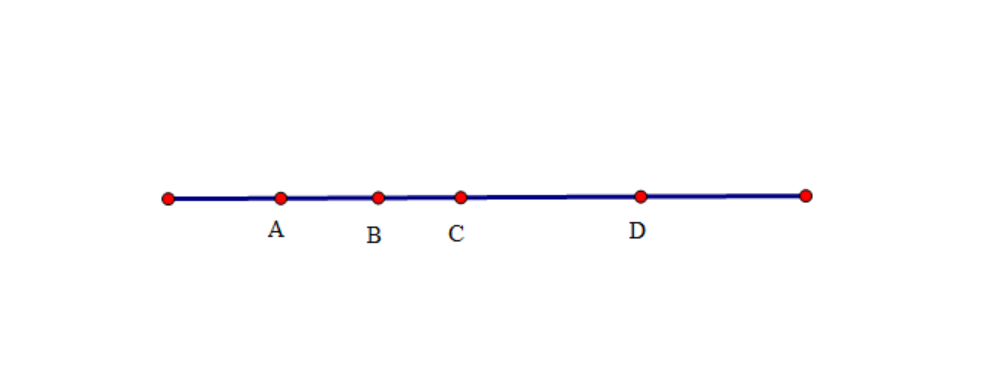
\includegraphics[scale=0.5]{figures/交比示意.png}
    \caption{交比示意图}
    \label{fig:p7}
\end{figure}
此处需要解释一下交比的定义。如图\ref{fig:p7}所示,直线上依次有ABCD四点,那么我们定义四个有序点的交比为:
\begin{equation}
    \frac{CA}{CB}/\frac{DA}{DB}
\end{equation}

\begin{figure}[H]
    \centering
    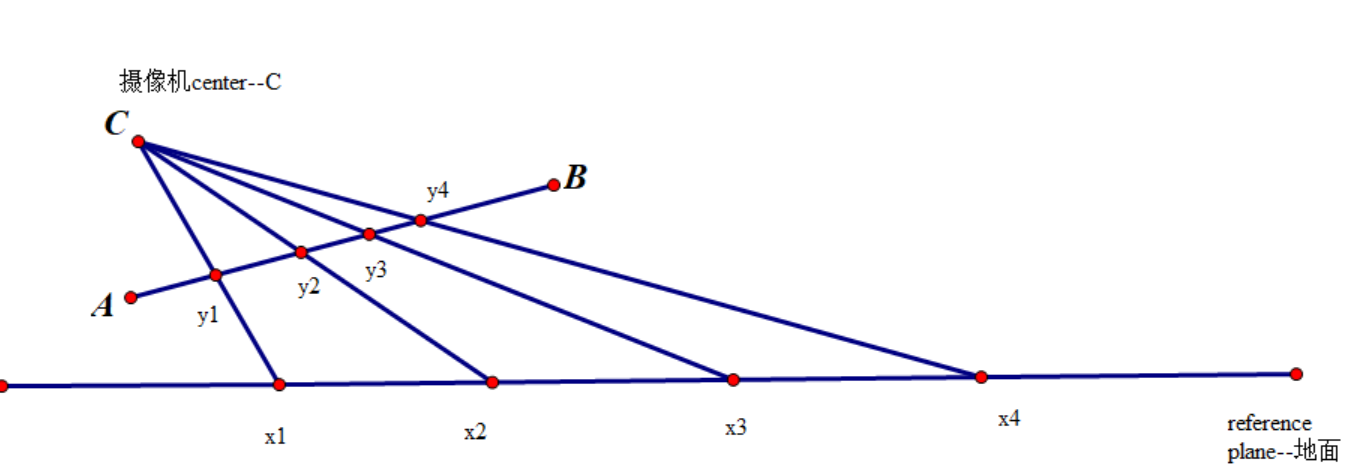
\includegraphics[scale=0.5]{figures/交比不变示意图.png}
    \caption{交比不变示意图}
    \label{fig:p8}
\end{figure}
如\ref{fig:p8}所示,C点为摄像机的中心点,AB可以认为是一张照片,水平线是地面,地面上选取在同一直线上的四个点$x1,x2,x3,x4$,在照片上成像时对应的点为$y1,y2,y3,y4$,交比不变的意思是,有如下等式成立:
\begin{equation}
    \begin{aligned}
        \frac{x3-x1}{x3-x2}/\frac{x4-x1}{x4-x2}=\frac{y3-y1}{y3-y2}/\frac{y4-y1}{y4-y2}
    \end{aligned}
\end{equation}
通过交比不变的性质,我们可以依据图像坐标系中的数据得到世界坐标系下的真实距离。下面我们演示一个例子。以\ref{fig:p4}的北口视频截图为例,计算停车线到图片下沿的长度。
\begin{figure}[H]
    \centering
    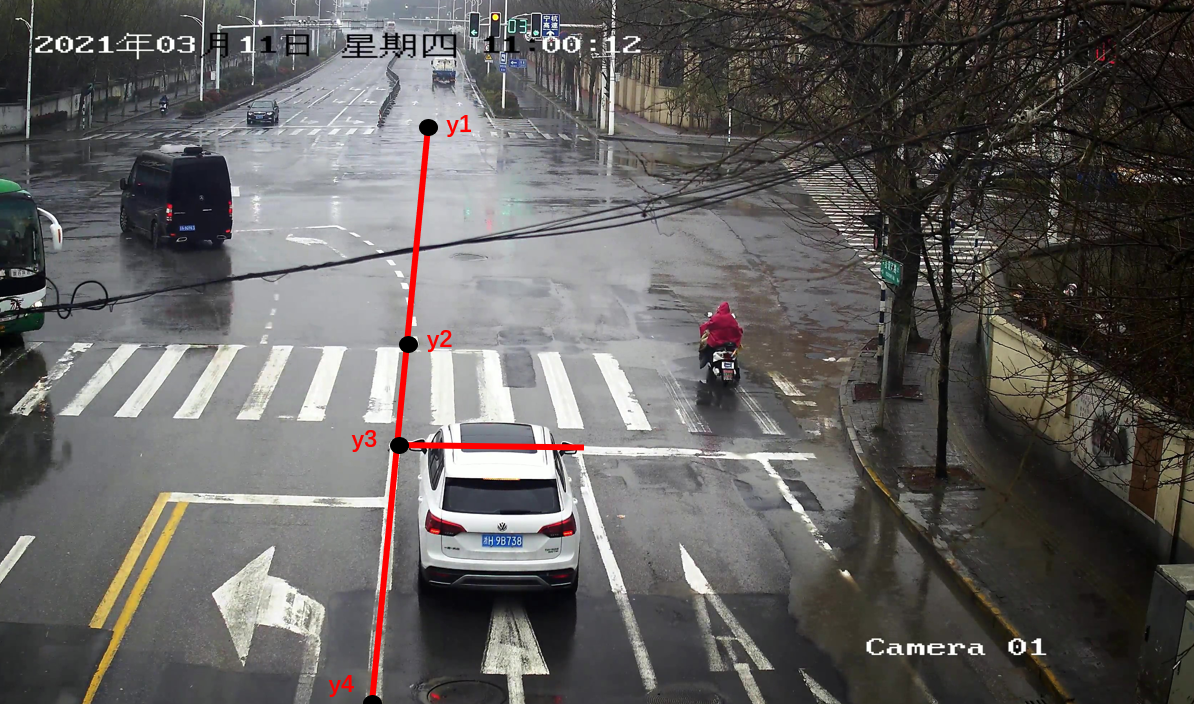
\includegraphics[scale=0.5]{figures/交比示例.png}
    \caption{交比示例}
    \label{fig:交比}
\end{figure}

如\ref{fig:交比}所示,此图为北口示意图,$y1y2$为北口斑马线顶端到南口停车线的图像上长度,$x1x2$为世界坐标系下的真实距离,42米。$y2y3$视为斑马线的图像长度,由于该路口确定,故斑马线长度$x2x3$确定,是3米。$y3y4$是停车线到图片底端的长度,$x3x4$是未知待求的。

\begin{figure}[H]
    \centering
    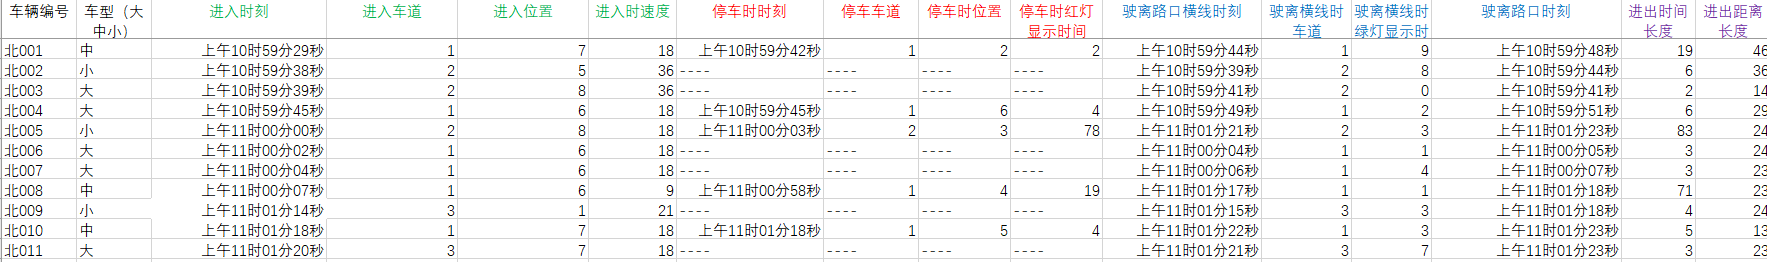
\includegraphics[scale=0.5]{figures/识别结果.png}
    \caption{识别结果}
    \label{fig:识别结果}
\end{figure}

\begin{figure}[H]
    \centering
    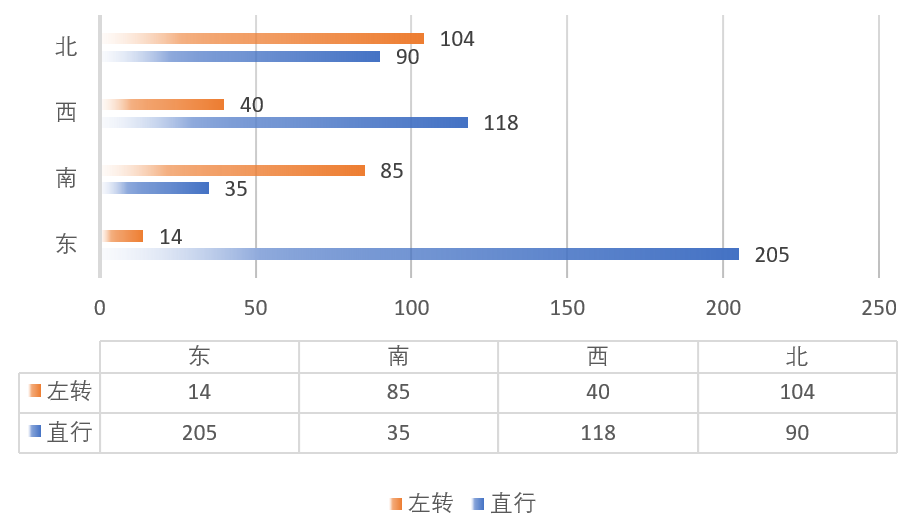
\includegraphics[scale=0.5]{figures/左转直行比例图.png}
    \caption{左转直行比例图}
    \label{fig:左转直行比例图}
\end{figure}

最终我们得到了如图\ref{fig:识别结果}所示结果,有些车的停车四列是虚线表示,代表该车没有等待信号灯,直接行驶了。驶离数据为空的数据行代表在视频周期内,车辆最终未能成功驶离。数据可视化表现为图\ref{fig:左转直行比例图}可以直观的看出东口西口的左转车辆相较南北左转相差悬殊,故二者的左转绿灯时间应该有相应的区别;同时东西的直行相较于南北的直行车辆较多,直行的绿灯应该更长。

    \section{问题二建模}
问题一提供了11:00:00至11:29:59在交叉路口驶入驶出车辆的时间、距离、位置等信息。在此基础上我们可以解决问题二。

\subsection{总流量和平均速度}

\subsubsection{定义与算法}
总流量:在采样时间段内驶离路口的车辆总数。

平均速度:各车辆行驶距离之和/各车辆行驶时间之和。

总流量只需,将所有驶离数据不为空的车辆计数加和即可,北口有194辆车通行,一辆未驶离;南口120辆均驶离;东口219辆,2辆未驶离;西口205辆,3辆未驶离。总流量为732辆。

平均速度的计算通过统计数据的进出时间长度求和/进出时间求和,即可得\textcolor{red}{总流量}。

\subsection{阻碍交通情况}

\subsubsection{道路概况}

下面引入一下交通问题中常用的变量及解释:


绿信比:绿信比是一个信号相位的有效绿灯时长与周期总时长之比。

信号周期:信号灯的各种灯色轮流显示一次所需要的时间。通常规定最短周期时间不得少于36秒。当交通需求较小时,信号周期则应较短,但一般不能小于P*15秒(P为相位数),以保证某一方向车辆及时安全通过路口。

进口道饱和流量:在一次连续的绿灯时间内,交叉口进车道上车队能够连续通过停车线的最多车辆数。

首先统计了信号灯的相位图,如下\ref{fig:p10}所示:
\begin{figure}[H]
    \centering
    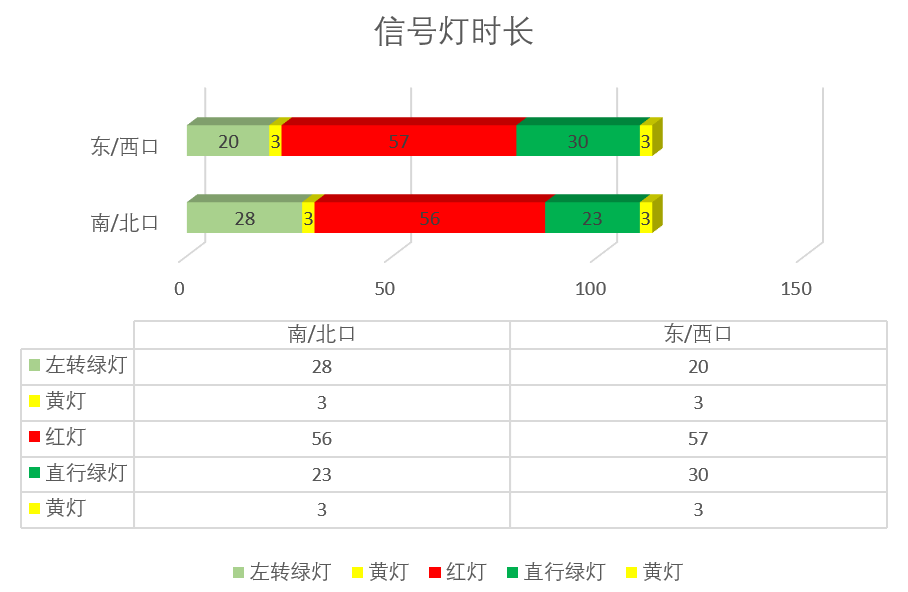
\includegraphics[scale=0.5]{figures/信号灯时长相位图.png}
    \caption{信号灯时长相位图}
    \label{fig:p10}
\end{figure}

东西方向与南北方向的信号周期均为113s,但显然信号灯的时长已经根据东西方向和南北方向车流量的不同进行了调整。南北方向左转车辆可能较多,东西方向直行车辆更多。这一特征可以在视频中显现。南北口的左转车辆略多于直行车辆,东西口则相反。同时也比较容易观察出的是北口车辆流量较大,其余路口车流稀少。

在我们查阅的论文中,对交叉路口交通信号优化控制,通常有以下2种角度:

(1)对信号周期进行优化;

(2)对相位信号(绿信比)进行优化;

我们若研究阻碍交通情况,也可以从这两个角度思考先考虑是不是信号周期整体时长不合理,无论是红灯还是绿灯都存在时长略长的情形;其次是考虑绿信比是否可以优化。此处我们作简要的说明,以北口11点钟的浙 98**8为例,在红灯倒计时56到38时,东西方向的停车等待的车辆大部分行驶完毕,剩下部分正好赶上绿灯而通行的车辆数量很少,那么直行的绿灯还有约10秒是被浪费了,对应的东西方向的绿灯时长过长,也代表着南北方向的红灯过长,故周期是不合理的,需要进行调整。相比之下,北口的车流量较大,直行和左转的时长基本恰好可以把等待的车辆放行结束。

通过观察可以发现,在路口通行的时候,无论是直行还是左转,大部分车辆都是在停车区或者待转区等待的车辆,恰好赶上绿灯的车辆为少数。也就是说,红灯的存在使得一部分车辆短暂停留在停车线,绿灯放行时,大部分车辆为等待的车辆,恰逢绿灯正常行驶的车辆是少数情况。\textcolor{red}{通过数据也可以观察出来,不需要停车的车辆比例相对于其他是很少的。(看数据再补全)}

\subsubsection{定义及结果}
本文对阻碍交通情况的定义为,在已经具备车辆正常通过路口的实时条件时,因为信号灯的存在而导致车辆不得不停车等待的情况为阻碍交通的情况。东西方向的车在绿灯时间内行驶结束,路口车辆被清空,南北方向的车辆理应正常行驶,但是需要等待红灯结束。同时也包含直行车辆清空,左转车辆仍需等待红灯才能左转的情形。


\begin{figure}[H]
    \centering
    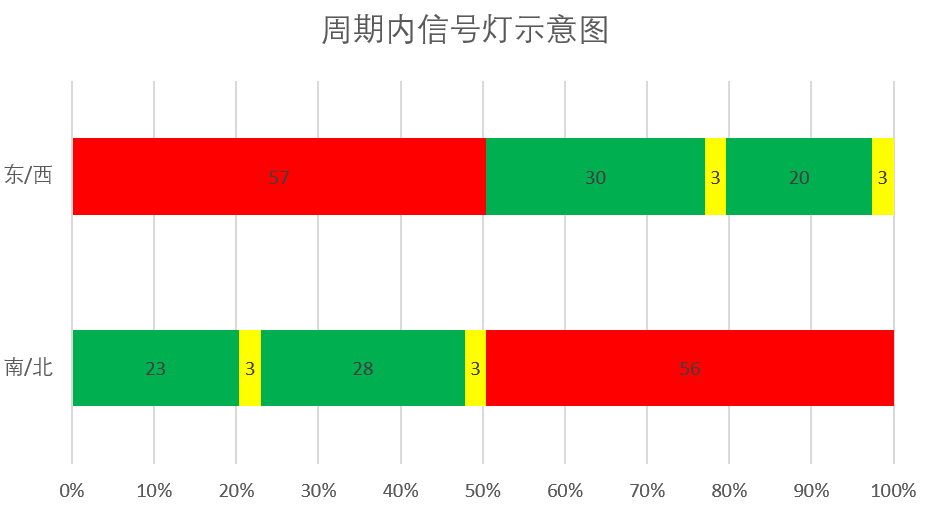
\includegraphics[scale=0.5]{figures/单周期信号灯示意图.png}
    \caption{单周期信号灯示意图}
    \label{fig:单周期}
\end{figure}

阻碍交通总时间的计算方法如下:
首先确定一个信号灯周期,分周期考虑每个周期内的阻碍交通时长,同时每个周期认为是相互独立此处以南北方向的直行绿灯亮起作为周期起点,具体示意如下\ref{fig:单周期},通过对周期进行划分,认为周期相互独立,再考虑各个周期内的阻碍时间的计算方法。

在最初级的处理中,我们只考虑临近时间区间的阻碍情况,例如东西方向的左转若有绿灯时间剩余,那么算作阻碍南北方向的直行;如果南北方向的直行绿灯有剩余,算作阻碍南北方向的左转;继而南北方向的左转会阻碍东西方向的直行。我们不考虑跨时间段阻碍,如果有车辆在南北方向红灯开始时就在左转停车区等待,那么东西方向的直行不仅会阻碍南北方向的直行,同时也会加长南北方向左转车辆的等待。但这种情况我们不考虑,只考虑直接相邻的时间区间的影响。

在计算阻碍时长的过程中,我们依次进行如下步骤:(1)记录南北方向直行车道,双向中最后一辆车辆驶离横线时的绿灯显示时间,记为$t1$,该时间算作阻碍南北方向左转车辆的时间;分别计算南北方向上自周期开始时至最后一辆车驶离时刻停留的车辆数,记为$x1$,$x_1\times t_1$则为南北方向直行阻碍南北方向左转的时间。
(2)记录南北方向左转双向车道中,最后一辆车驶离横线时绿灯显示时间,记为$t_2$, 该时间作为阻碍东西方向直行的车辆的阻碍时间;计算自周期开始时至最后一辆车左转驶离时刻时间内,停留的车辆数,记为$x_2$,用$x_2 \times t_2$作为南北方向左转阻碍东西方向直行的时间。
重复1、2步骤,但是是在计算东西方向的直行阻碍最左转,和东西方向左转阻碍南北方向直行。

对于车辆,在一个周期中,绿灯的主要放行目标定为,在红灯时刻到达等待绿灯的车辆。考虑“驶离横线时绿灯示数”这一指标,考虑同一周期内,同向行驶车辆,车辆行驶数量过半时,首次出现同向两车示数差异大于5秒以上,将前者剩余绿灯时间进行标记,调查其驶离路口时刻,该时刻认为不阻碍交通的绿灯开始时刻,考虑同时搜寻在另外方向上停车等待车辆。
车辆行驶玩
    \section{问题三建模}
在问题三中,我们需要根据第一问中以获得的车辆相关信息,对目前为机械方案的红绿灯配时进行优化,在不同的子时间段进行实时地适应性调节,设定更加合理的周期与配时。优化算法考虑**

此外还要在原有车辆信息基础上,利用优化后的时间数据,对车辆通行情况进行仿真模拟,重新统计得到优化后的基本信息。

基本假设:

(1)有车辆在行驶过程中,无突发事故影响正常行驶

(2)交通信号灯均按照配时方案正常工作

(3)忽略行人、非机动车的行动对车辆行驶的影响

\subsection{现有方案分析}

\subsubsection{机械配时方案}
通过提取所给场景中的信号灯变化信息,提取出初始机械配时周期,东西方向全红灯(可右行)亮57秒,直行(可右转)绿灯亮30秒,黄灯亮3秒,左转(可右转)绿灯亮20秒,黄灯再亮3秒;南北方向全红灯亮56秒,仅直行绿灯亮23秒,黄灯亮3秒,左转(可右转)绿灯亮28秒,黄灯再亮3秒,该周期共113秒。东西方向全红灯开始时间与南北方向直行绿灯亮起时间保持一致,因此一周期内的全红时间为0。

\subsubsection{优化方案初设}
根据车辆信息进一步整理分析发现,目前车辆比较稀少,存在着明显的阻碍交通情况:南北/东西方向有车辆需要通行,可是南北/东西方向亮着红灯,而东西/南北方向亮着绿灯,不同时间段存在着不等长的道路空白期。故根据不同方向上被阻碍时间的长短进行划分,构成待优化的三组子时间段,利用优化方法分别进行优化。

\textcolor{red}{表格表格表格表格表格表格表格表格表格表格表格}

\subsection{信息提取}

\subsubsection{相位方案}
信号相位指交通信号灯给各方向的车辆轮流分配通行权的信号显示,通过观察现有四相位方案下右转车道基本保持通畅,因此考虑基于直行与左转绿灯的四相位优化方案。相位方案如下图所示:

\textcolor{red}{图图图图图图图图图图图图图图图图图图图图图图}

\subsubsection{交通流量折算}
模型中用到多个关于车流量的变量,单位为pcu,指标准车当量数,又称当量交通量。对各种各样的实际车辆按《城市道路设计规范》中规定的折算系数折算系数换算成某种标准车型的当量交通量。数据中涉及到的车型对应折算比例为:小型车1.0,大客车、中型货车1.5,大型货车2.0。

\subsubsection{车道饱和流量校正}
基本饱和流量信息参考中国城市车道平均水平,记为$S_{ave}$直行车道1650pcu/h,右转车道1450pcu/h,左转车道1550pcu/h,按照道路信息进行宽度校正,转弯半径校正。宽度校正系数$f_w$在2.8m时为$0.4*(2.8-0.5)$,3.2m时为1。转弯半径校正系数$f_r$,依照提取出的转弯半径信息,在左转时为1,右转时为0.97。可得到实际车道饱和流量$S=S_{ave}*f_w*f_r$。

\subsection{目标函数建立}

\subsubsection{平均延误时间}
延误时间表示车辆受阻情况下通过岔路口的时间和正常行驶通过的时间差,由一致性延误$d_{u}$描述到达率为常数的延误和随机延误$d_{r}$此时到达率不为常数,两部分组成。计算方法分别如下:
\begin{equation}
    d_{ui}=\sum_{j} \frac{c\left(1-g_{i} / c\right)^{2}}{2\left(1-y_{i j}\right)}
\end{equation}
\begin{equation}
    d_{ri}=\sum_{j} \frac{y_{i j}^{2}}{2 q_{i j}\left(1-y_{i j}\right)}
\end{equation}
\begin{equation}
    d_{i}=d_{ui}+d_{ri}
\end{equation}
其中$i = 1,2,3,4$表示四个相位,$j=1,2,3,4$表示四个车道;$d_i$表示第i相位平均延误;$c$为周期长信号灯各色完整显示所花时间,这里为113s;$g_i$表示第i相位有效绿灯时长,$q_{ij}$表示第i相位第j车道进口当前流量值pcu/h;$y_{ij}$表示第i相位第j车道进口交通强度,即实际流量值和饱和流量值的比值。因此一周期内的平均延误为各相位延误加权平均值,计算公式为:$\sum_{i} d_i q_{i} /\sum_{i} q_{i}$,其中$q_{i}=\sum_{j} q_{ij}$。

\subsubsection{进入速度损失}
由于车辆停车的可能性与交通饱和率成反比,参考文献知车辆的平均停车次数可由              \begin{equation}
                                                      w_{i}=\sum_{j} 0.9 \frac{\left(c-g_{i}\right)}{1-y_{i j}}
\end{equation}
估计,因此对应第i相位所有进入车辆产生的平均速度$v_i$,通过实际计算采用$v_i'=v_i/10$作为速度加权因子,得到各相位速度损失加权平均值:$\sum_{i}v_i h_i q_{i} /\sum_{i} q_{i}$。

\subsubsection{通行能力}
通行能力用于表示车辆在有效绿灯时间通过停车线的数目,根据交通管理与控制标准计算方法求得
\begin{equation}
    z_{i}=\frac{s_{i} \times g_{i}}{c}
\end{equation}
$s_i$为第i条进口车道的饱和流量。在此基础上进行相位加权得:$\sum_{i} z_i q_{i} /\sum_{i} q_{i}$

\subsubsection{目标函数与约束条件}
为使车辆通过路口的平均速度最大,以延误时间最短,进入速度损失最小,通行能力最大为目标。利用罚函数的思想建立了如下目标函数
\begin{equation}
    \min _{X} f(X)=\sum_{i}( k_{i}^{1} d_{i}+k_{i}^{2} w_{i}-k_{i}^{3} z_{i})
\end{equation}
其中$k_{i}^{1}, k_{i}^{2}, k_{i}^{3}$系数设置参考\textcolor{red}{14,15},对应计算方法为$k_{i}^{1}=2(1.0-Y) \times \sqrt[7]{s_{i}}$,$ k_{i}^{2}=\sqrt[7]{s_{i}} \times \frac{1.0-Y}{0.9}$,$k_{i}^{3}=2 Y \times \frac{c}{3600}$。其中$Y=\sum \operatorname{max}y_{ij}$。

约束条件为周期时间约束,饱和度约束等,具体表达式如下:
$$C_{\min } \leqslant C \leqslant C_{\max }$$
$$\sum_{i} (g_{i}+t_{l})=C$$
$$0.7 \leqslant \frac{y_{i} c}{g_{i}} \leqslant 0.9,1 \leqslant i \leqslant n$$
$$g_{i} \in Z^{+}, 1 \leqslant i \leqslant n$$
0.7用来避免在饱和度过小,即通行能力远大于需求,增加车辆阻碍,0.9用来避免饱和度过大而造成堵塞。$t_l$表示每相损失时间,由启动损失时间$t_{l1}$和清尾损失$t_{l2}$分组成,停车等待的车辆在绿灯开始时不能立即提高速度,存在时间损失$t_{l1}$,一般为2s,清尾损失$t_{l2}$表示黄灯时间,这里为3s。故,$t_l=5s$。

\subsection{优化算法与结果展示}

\subsubsection{Webster时配算法}
韦伯斯特(Webster)算法以降低交叉口车辆延误为目标,进行配时优化的经典算法。通过大量现场交通观察,结合排队论和计算机模拟得出的算法。在单点信号配时、平峰路口优化方面效果良好,与文中所示情况相符。运用近似解法,得到最佳周期时长为
\begin{equation}
    c_{0}=\frac{1.5 L+5}{1-Y}
\end{equation}
最佳有效绿灯时长为
\begin{equation}
    g_{i}=(c_{0}-t_l*4)\frac{y_i}{\sum_{i} y_{i}}
\end{equation}

\subsubsection{遗传算法}
遗传算法是一种效率较高的参数寻找最优解的算法,参考仿生原理快速搜索解空间,因此适用于该问题关于交通系统时间配置的优化问题。
算法基本步骤如下:(1)设置如种群大小、交叉概率等的基本参数;(2) 对问题进行实数编码,用解数据表示基因型串结构数据;(3)随机生成串行结构初值作为初始种群;(4)基于动态函数惩罚法来构造适应度函数:$F(x)=\frac{1}{\varepsilon+f(x)}$;(5) 适应度比例的选择采用轮盘赌方法;(6)采用取自$[0,1]$的随机数的实数交叉法;(7)采用非均匀变异对原有基因进行小范围扰动;(8)记录结果,进行判断是否需要进行下一次迭代。

\subsubsection{优化配时方案}
通过数据计算可知,现有配时对应平均延误较大,主要原因在于相位交通流量与对应时间存在差距。

利用Webster配时法计算得出修正方案:

遗传算法中的参数设置如下:最大遗传代数为500,初始种群大小为100,交叉率为0.8,染色体长为5,变异率为0.01。

\subsection{仿真实验}

\subsubsection{车流模拟}
在仿真试验中,车辆以表一中的车辆进入相关信息编制车辆行驶算法,使车辆在红绿灯相位在对应的车道执行停车等待,启动离开的行驶动作,所有车辆在黄灯开始时不超越停车线。在此基础上添加动态算法,防止车辆与车辆之间的碰撞。

\subsubsection{优化结果对比}
从计算机视觉的视角,一张图片我们需要考虑多个坐标系:

    \newpage
    \bibliographystyle{acm}
    \bibliography{ref}
\end{document}